\chapter{Constructions}
\label{chap:constructions}

In this chapter we explore some basic constructions in categories. We
shall use these constructions for describing some concepts and
examples in all the following chapters.

\section{Isomorphisms}
\label{sec:constructions-isomorphisms}

We shall often find the concept of isomorphism and the property of
uniqueness up to isomorphism.

\begin{definition}
  \label{def:isomorphism}

  %% \parencite[15]{pierce-1991}

  Let $\cat{C}$ be a category. A morphism $f: a \to b$ is an
  isomorphism if there is an inverse morphism $f^{-1}: b \to a$ such
  that
  \begin{equation}
    \label{eq:isomorphism}
    f^{-1} \comp f = \idO{a}
    \quad
    \text{and}
    \quad
    f \comp f^{-1} = \idO{b}
    \text{.}
  \end{equation}
  Objects $a$ and $b$ are isomorphic if there is an isomorphism $f: a
  \to b$. Isomorphic objects are often said to be identical up to
  isomorphism. Similarly, an object with some property is said to be
  unique up to isomorphism if every object satisfying the property is
  isomorphic to it.

\end{definition}

\section{Initial and Terminal Objects}
\label{sec:constructions-initial-terminal-objects}

We define initial and terminal objects, which we shall use for
describing algebras and initial algebras.

\begin{definition}
  \label{def:initial-object}

  %% \parencite[444]{poigne-1992}

  Let $\cat{C}$ be a category. An object $0$ is the initial object of
  $\cat{C}$ if, for all objects $a$, there is a unique morphism $0 \to
  a$.

\end{definition}

\begin{definition}
  \label{def:terminal-object}

  %% \parencite[439]{poigne-1992}

  Let $\cat{C}$ be a category. An object $1$ is the terminal object of
  $\cat{C}$ if, for all objects $a$, there is a unique morphism $a \to
  1$.

\end{definition}

\begin{lemma}

  Initial and terminal objects are unique up to isomorphism.

  \begin{proof}

    Let $\cat{C}$ be a category with initial objects $0$ and $0'$.
    There are unique morphisms $0_{0'}: 0 \to 0'$ and $0'_{0}: 0' \to
    0$, and $0_{0} = \idO{0}$ and $0'_{0'} = \idO{0'}$. Hence, $0'_{0}
    \comp 0_{0'} = \idO{0}$ and $0_{0'} \comp 0'_{0} = \idO{0'}$. That
    is, $0$ is unique up to isomorphism.

    Similarly, let $\cat{C}$ be a category with terminal objects $1$
    and $1'$. There are unique morphisms $1_{1'}: 1' \to 1$ and
    $1'_{1}: 1 \to 1'$, and $1_{1} = \idO{1}$ and $1'_{1'} =
    \idO{1'}$. Hence, $1_{1'} \comp 1'_{1} = \idO{1}$ and $1'_{1}
    \comp 1_{1'} = \idO{1'}$. That is, $1$ is unique up to
    isomorphism.

  \end{proof}

\end{lemma}

As examples, we consider initial and terminal objects in the
categories \set, \hask, and \agda.

\begin{example}
  \label{ex:initial-terminal-objects-set}

  %% \parencite[16]{pierce-1991}

  In \set, the empty set $\emptyset$ is the initial object. Given a
  set $A$, the empty function is the unique function $\emptyset \to
  A$. Additionally, any singleton set $\{x\}$ is a terminal object.
  Given a set $A$, the function which assigns $x$ to each element of
  $A$ is the unique function $A \to \{x\}$.

\end{example}

\begin{example}
  \label{ex:initial-terminal-objects-haskell}

  In \hask, the empty or uninhabited type is the initial object of the
  category:
  \begin{codehaskell}
data Void
  \end{codehaskell}
  The \texthaskell{absurd} function, as defined, for instance, in
  \parencite{kmett-2012}, is the unique function required to show that
  \texthaskell{Void} is indeed the initial object:
  \begin{codehaskell}
absurd :: Void -> a
absurd = absurd
  \end{codehaskell}
  Note that, in the absence of Convention \ref{con:hask}, we would
  also have:
  \begin{codehaskell}
absurd' :: Void -> a
absurd' _ = undefined
  \end{codehaskell}
  Additionally, the unit type is the terminal object of the category:
  \begin{codehaskell}
data () = ()
  \end{codehaskell}
  The \texthaskell{unit} function is the unique function required to
  show that \texthaskell{()} really is the terminal object:
  \begin{codehaskell}
unit :: a -> ()
unit _ = ()
  \end{codehaskell}
  Without Convention \ref{con:hask}, we would also have:
  \begin{codehaskell}
unit' :: a -> ()
unit' _ = undefined
  \end{codehaskell}

\end{example}

\begin{example}
  \label{ex:initial-terminal-objects-agda}

  In \agda, the empty type, defined in \module{Data.Empty}, is the
  initial object:
  \begin{codeagda}
data ⊥ : Set where
  \end{codeagda}
  The \textagda{⊥-elim} function, defined in \module{Abel.Data.Empty},
  is the unique function required to show that \textagda{⊥} is indeed
  the initial object:
  \begin{codeagda}
⊥-elim : {A : Set} → ⊥ → A
⊥-elim ()
  \end{codeagda}
  The unit type, defined in \module{Data.Unit}, is the terminal
  object:
  \begin{codeagda}
record ⊤ : Set where
  constructor tt
  \end{codeagda}
  Or, equivalently, the unit type defined in \module{Data.Unit.Core}:
  \begin{codeagda}
data Unit : Set where
  unit : Unit
  \end{codeagda}
  Finally, the \textagda{unit} function, defined in
  \module{Abel.Data.Unit}, is the unique function required to show
  that \textagda{Unit} really is the terminal object:
  \begin{codeagda}
unit : {A : Set} → A → ⊤
unit _ = tt
  \end{codeagda}

\end{example}

\begin{example}
  \label{ex:terminal-objects-constants}

  %% \parencite[16--17]{pierce-1991}

  In \set, the elements of a set $A$ can be considered as functions
  from a terminal object, that is, any singleton set, to $A$. More
  specifically, if $x \in A$ and $1$ is a terminal object, then $x$
  can be considered as a function $x: 1 \to A$ which assigns $x$ to
  the element of $1$.

\end{example}

\section{Products and Coproducts}
\label{sec:constructions-products-coproducts}

In this section, we describe the concepts of product and coproduct,
which correspond to Cartesian products and disjoint unions,
respectively. As examples, we consider both constructions in the
categories \set, \hask, and \agda.

\begin{definition}
  \label{def:product}

  %% \parencite[18]{pierce-1991}

  A product of objects $a$ and $b$ in a category \cat{C} consists of a
  product object $a \times b$, and projection morphisms $\pi_{1}: a
  \times b \to a$ and $\pi_{2}: a \times b \to b$, such that, for all
  objects $c$, and morphisms $f: c \to a$ and $g: c \to b$, there is a
  unique morphism $\langle{f,g}\rangle: c \to a \times b$ such that
  \begin{equation}
    \label{eq:product}
    \pi_{1} \comp \langle{f,g}\rangle = f
    \quad
    \text{and}
    \quad
    \pi_{2} \comp \langle{f,g}\rangle = g
    \text{,}
  \end{equation}
  that is, the diagram in Figure \ref{fig:product} is commutative.

  \begin{figure}[htb]
    \begin{center}
      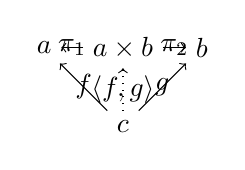
\begin{tikzpicture}
        \node (axb)               {$a \times b$};

        \node (a)  [left of=axb]  {$a$};
        \node (b)  [right of=axb] {$b$};
        \node (c)  [below of=axb] {$c$};

        \draw [->] (axb) to node [swap] {$\pi_{1}$} (a);
        \draw [->] (axb) to node        {$\pi_{2}$} (b);

        \draw [->] (c)  to node        {$f$} (a);
        \draw [->] (c)  to node [swap] {$g$} (b);

        \draw [->,dotted] (c)  to node [swap] {$\langle{f,g}\rangle$} (axb);
      \end{tikzpicture}
    \end{center}
    \caption{A product.}
    \label{fig:product}
  \end{figure}

\end{definition}

\begin{example}
  \label{ex:product-set}

  %% \parencites[439--440]{poigne-1992}[17--18]{pierce-1991}

  In \set, the product of two sets $A$ and $B$ consists of the
  Cartesian product
  \begin{equation}
    A \times B = \{(x,y) \mid x \in A \quad\text{and}\quad y \in B\}
    \text{,}
  \end{equation}
  and two projection functions $\pi_{1}: A \times B \to A$ and
  $\pi_{2}: A \times B \to B$ such that, for all $(x,y) \in A \times
  B$,
  \begin{equation*}
    \pi_{1}(x,y) = x
    \quad
    \text{and}
    \quad
    \pi_{2}(x,y) = y
    \text{.}
  \end{equation*}
  Given a set $C$, and two functions $f: C \to A$ and $g: C \to B$,
  there is a unique function $\langle{f,g}\rangle: C \to A \times B$
  defined by
  \begin{equation*}
    \langle{f,g}\rangle(z) = (f(z),g(z))
  \end{equation*}
  for all $z \in C$. Equations \eqref{eq:product} hold.

\end{example}

\begin{example}
  \label{ex:product-haskell}

  In \hask, tuples are products:
  \begin{codehaskell}
data (,) a b = (,) a b
  \end{codehaskell}
  The projection functions are \texthaskell{fst} and
  \texthaskell{snd}, which extract the first and second components of
  a pair, respectively:
  \begin{codehaskell}
fst :: (a,b) -> a
fst (x,_) = x

snd :: (a,b) -> b
snd (_,y) = y
  \end{codehaskell}
  The \texthaskell{fork} function is the function required to show
  that tuples are indeed products:
  \begin{codehaskell}
fork :: (c -> a) -> (c -> b) -> c -> (a,b)
fork f g z = (f z,g z)
  \end{codehaskell}

\end{example}

\begin{example}[See module \module{Abel.Data.Product}]
  \label{ex:product-agda}

  In \agda, products and their projection functions are defined as
  follows:
  \begin{codeagda}
data _×_ (A B : Set) : Set where
  _,_ : A → B → A × B

proj₁ : {A B : Set} → A × B → A
proj₁ (x , _) = x

proj₂ : {A B : Set} → A × B → B
proj₂ (_ , y) = y
  \end{codeagda}
  The required function to satisfy the definition of products is:
  \begin{codeagda}
⟨_,_⟩ : {A B C : Set} → (C → A) → (C → B) → C → A × B
⟨_,_⟩ f g z = f z , g z
  \end{codeagda}

\end{example}

\begin{definition}
  \label{def:coproduct}

  %% \parencite[19]{pierce-1991}

  A coproduct of objects $a$ and $b$ in a category \cat{C} consists of
  a coproduct object $a + b$, and injection morphisms $\iota_{1}: a
  \to a + b$ and $\iota_{2}: b \to a + b$, such that, for all objects
  $c$, and morphisms $f: a \to c$ and $g: b \to c$, there is a unique
  morphism $[f,g]: a + b \to c$ such that
  \begin{equation}
    \label{eq:coproduct}
    [f,g] \comp \iota_{1} = f
    \quad
    \text{and}
    \quad
    [f,g] \comp \iota_{2} = g
    \text{,}
  \end{equation}
  that is, the diagram in Figure \ref{fig:coproduct} is commutative.

  \begin{figure}[htb]
    \begin{center}
      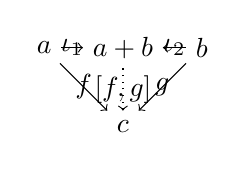
\begin{tikzpicture}
        \node (a+b) {$a + b$};

        \node (a) [left of=a+b]  {$a$};
        \node (b) [right of=a+b] {$b$};
        \node (c) [below of=a+b] {$c$};

        \draw [<-] (a+b) to node [swap] {$\iota_{1}$} (a);
        \draw [<-] (a+b) to node        {$\iota_{2}$} (b);

        \draw [<-] (c) to node        {$f$} (a);
        \draw [<-] (c) to node [swap] {$g$} (b);

        \draw [<-,dotted] (c) to node [swap] {$[f,g]$} (a+b);
      \end{tikzpicture}
    \end{center}
    \caption{A coproduct.}
    \label{fig:coproduct}
  \end{figure}

\end{definition}

\begin{example}
  \label{ex:coproduct-set}

  %% \parencite[63]{maclane-1998}

  In \set, the coproduct of two sets $A$ and $B$ consists of the
  disjoint union
  \begin{equation}
    A + B = (\{1\} \times A) \cup (\{2\} \times B)
    \text{,}
  \end{equation}
  and two injection functions $\iota_{1}: A \to A + B$ and $\iota_{2}:
  B \to A + B$ such that, for all $x \in A$ and $y \in B$,
  \begin{equation}
    \iota_{1}(x) = (1,x)
    \quad
    \text{and}
    \quad
    \iota_{2}(y) = (2,y)
    \text{.}
  \end{equation}
  Given a set $C$, and two functions $f: A \to C$ and $g: B \to C$,
  there is a unique function $[f,g]: A + B \to C$ defined by
  \begin{equation}
    [f,g](\iota_{1}(x)) = f(x)
    \quad
    \text{and}
    \quad
    [f,g](\iota_{2}(y)) = g(y)
  \end{equation}
  for all $x \in A$ and $y \in B$. Equations \eqref{eq:coproduct}
  hold.

\end{example}

\begin{example}
  \label{ex:coproduct-haskell}

  In \hask, coproducts and their injection functions are defined by
  the \texthaskell{Either} type:
  \begin{codehaskell}
data Either a b = Left a | Right b
  \end{codehaskell}
  The \texthaskell{either} function is the function required to
  satisfy the definition of a coproduct:
  \begin{codehaskell}
either :: (a -> c) -> (b -> c) -> Either a b -> c
either f _ (Left x)  = f x
either _ g (Right y) = g y
  \end{codehaskell}

\end{example}

\begin{example}[See module \module{Abel.Data.Sum}]
  \label{ex:coproduct-agda}

  In \agda, sums or disjoint unions are coproducts:
  \begin{codeagda}
data _+_ (A B : Set) : Set where
  inj₁ : (x : A) → A + B
  inj₂ : (y : B) → A + B
  \end{codeagda}
  Finally, the required function to show that sums are indeed
  coproducts is defined as follows:
  \begin{codeagda}
[_,_] : {A B C : Set} (f : A → C) (g : B → C) → A + B → C
[_,_] f _ (inj₁ x) = f x
[_,_] _ g (inj₂ y) = g y
  \end{codeagda}

\end{example}

\section{References}
\label{sec:constructions-references}

This chapter is based on \parencites[15--19]{pierce-1991}[439--440,
  444]{poigne-1992}[63]{maclane-1998}.

\clearemptydoublepage
